\documentclass[review]{elsarticle}

\usepackage{lineno}
\usepackage{xspace}
\modulolinenumbers[5]

\journal{Journal}

%% `Elsevier LaTeX' style
\bibliographystyle{elsarticle-num}
%%%%%%%%%%%%%%%%%%%%%%%

%%%% packages and definitions (optional)
\usepackage{placeins}
\usepackage{booktabs} % nice rules (thick lines) for tables
\usepackage{microtype} % improves typography for PDF
\usepackage{hhline}
\usepackage{amsmath}

%\usepackage[demo]{graphicx}
%\usepackage{caption}
%\usepackage{subcaption}

\usepackage{booktabs}
\usepackage{threeparttable, tablefootnote}
\usepackage{floatrow}
\usepackage{subcaption}
\usepackage{multirow}

\usepackage{tabularx}
\newcolumntype{b}{>{\hsize=1.0\hsize}X}
\newcolumntype{s}{>{\hsize=.5\hsize}X}
\newcolumntype{m}{>{\hsize=.75\hsize}X}
\newcolumntype{x}{>{\hsize=.25\hsize}X}
\newcolumntype{L}{>{\raggedright\arraybackslash}X}
\newcolumntype{R}{>{\raggedleft\arraybackslash}X}
\def\arraystretch{1}

\graphicspath{{figures/}}

% tikz %
\usepackage{tikz}
\usetikzlibrary{positioning, arrows, decorations, shapes}

\usetikzlibrary{shapes.geometric,arrows}
\tikzstyle{process} = [rectangle, rounded corners, minimum width=3cm, minimum height=1cm,text centered, draw=black, fill=blue!30]
\tikzstyle{object} = [ellipse, rounded corners, minimum width=3cm, minimum height=1cm,text centered, draw=black, fill=green!30]
\tikzstyle{arrow} = [thick,->,>=stealth]

\definecolor{illiniblue}{HTML}{B1C6E2}
\definecolor{illiniorange}{HTML}{f8c2a2}
\usetikzlibrary{shapes.geometric, arrows}
\tikzstyle{oblock} = [rectangle, draw, fill=illiniorange, 
text width=15em, text centered, rounded corners, minimum height=4em]
\tikzstyle{bblock} = [rectangle, draw, fill=illiniblue, 
text width=15em, text centered, rounded corners, minimum height=4em]
\tikzstyle{arrow} = [thick,->,>=stealth]

% hyperref %
\usepackage[hidelinks]{hyperref}
% after hyperref %
\usepackage{cleveref}
\usepackage{datatool}
\usepackage[acronym,toc]{glossaries}
\include{acros}

\newcommand{\Cyclus}{\textsc{Cyclus}\xspace}%
\newcommand{\Cycamore}{\textsc{Cycamore}\xspace}%
\newcommand{\deploy}{\texttt{d3ploy}\xspace}%

\makeglossaries

\begin{document}
\begin{frontmatter}
\title{Demand Driven Deployment Capabilities in Cyclus, a Fuel Cycle Simulator}

\date{}                     %% if you don't need date to appear

%% Authors
\author[uiuc]{Gwendolyn J. Chee\corref{corrauthor}}
\author[uiuc]{Roberto E. Fairhurst Agosta}
\author[ornl]{Jin Whan Bae}
\author[usc]{Robert R. Flanagan}
\author[quan]{Anthony M. Scopatz}
\author[uiuc]{Kathryn D. Huff}
\cortext[corrauthor]{Corresponding Author}
\ead{gchee2@illinois.edu}


% Institutes of the authors
\address[uiuc]{Dept. of Nuclear, Plasma, and Radiological Engineering, University of Illinois at Urbana-Champaign, Urbana, IL 61801}
\address[ornl]{Oak Ridge National Laboratory, Oak Ridge, TN, United States}
\address[usc]{Nuclear Engineering Program, University of South Carolina}
\address[quan]{Quansight, LLC}
	
\begin{keyword}
nuclear fuel cycle \sep
python \sep 
time series forecasting
\end{keyword}

\begin{abstract}
The present United States nuclear fuel cycle faces challenges that hinder 
the expansion of nuclear energy technology. 
The U.S. Department of Energy identified four nuclear fuel cycle 
options we could transition to, which would make nuclear energy technology
more desirable. 
To successfully analyze the transition from our current 
fuel cycle to these promising fuel cycles, we need a nuclear 
fuel cycle simulator that can predictively and automatically 
deploy fuel cycle facilities to meet user-defined power demand. 
In this work, we developed demand-driven deployment capabilities in 
\Cyclus, a nuclear fuel cycle simulator.  
User-controlled capabilities such as supply buffers, 
facility preferences, prediction algorithms, and installed capacity 
deployment were introduced to give users tools to minimize power 
undersupply in a transition scenario simulation. 
We demonstrate \deploy's capability to automatically deploy fuel 
cycle facilities to set up transition scenarios for promising 
nuclear fuel cycle options. 
\end{abstract}



\end{frontmatter}
\glsresetall

\linenumbers

\section{Introduction}
The nuclear fuel cycle represents the nuclear fuel life cycle from initial
extraction through processing, use in reactors, and, eventually, 
final disposal.
This complex system of facilities and mass flows 
collectively provide nuclear energy 
in the form of electricity \cite{yacout_modeling_2005}.
Nuclear fuel cycle simulator tools were introduced to investigate 
nuclear fuel cycle dynamics at a local and global level. 
These simulators track the flow of materials through the nuclear fuel cycle, 
from enrichment to final disposal of the fuel, while also accounting for 
decay and transmutation of isotopes. 
The impacts are evaluated in the form of `metrics', quantitative measures 
of performance \cite{huff_fundamental_2016}. 
These metrics are calculated from mass balances and facility operation 
histories calculated by a fuel cycle simulator \cite{huff_fundamental_2016}. 
By evaluating performance metrics of different fuel cycles, we gain an 
understanding of how each facility's parameters and technology choices 
impact the system's performance. 
Therefore, these results can be used to guide research 
efforts, advise future design choices, and provide 
decision-makers with a transparent tool for evaluating \gls{FCO} 
to inform big-picture policy decisions \cite{yacout_modeling_2005}.

Many fuel cycle simulators automatically deploy reactor facilities 
to meet a user-defined power demand. 
However, the user must define a deployment scheme of 
supporting facilities to avoid gaps in the supply 
chain resulting in idle reactor capacity. 
Current simulators require the user to set infinite capacity 
for supporting facilities but this inaccurately represents 
reality and obfuscates required capacities. 
Manually determining a deployment scheme for a once-through 
fuel cycle is straightforward, however, for complex fuel cycle 
scenarios, it is not.   
To ease setting up realistic nuclear fuel cycle simulations, a nuclear fuel cycle simulator
must bring dynamic demand-responsive deployment decisions into 
the simulation logic \cite{huff_current_2017}. 
This means the nuclear fuel cycle simulator decides how many mines, 
mills, enrichment facilities,
reprocessing facilities, etc are deployed to support dynamically 
changing power demand and reactor types.  
Thus, a next-generation nuclear fuel cycle simulator must predictively and 
automatically deploy fuel cycle facilities to meet a user-defined 
power demand. 

In \Cyclus, an agent-based nuclear fuel cycle simulation framework 
\cite{huff_fundamental_2016}, 
each entity (i.e. \texttt{Region}, \texttt{Institution}, or \texttt{Facility}) in the 
fuel cycle is an agent. 
\texttt{Region} agents represent geographical or political areas in which \texttt{Institution}
and \texttt{Facility} agents reside. 
\texttt{Institution} agents represent legal operating organizations such as
utilities, governments, and control the 
deployment and decommissioning of \texttt{Facility} agents
\cite{huff_fundamental_2016}.
\texttt{Facility} agents represent nuclear fuel cycle facilities
such as mines, conversion facilities, reactors, reprocessing facilities, 
etc. 
\Cycamore \cite{carlsen_cycamore_2014}
provides basic \texttt{Region}, \texttt{Institution}, 
and \texttt{Facility} archetypes compatible with \Cyclus. 

\subsection{Context of Work}
The impact of climate change on natural and human systems 
is increasingly apparent.
The production and use of energy contribute to 
two-thirds of the total Green House Gas (GHG) 
emissions \cite{noauthor_climate_2018}.
Furthermore, as the human population increases and previously 
under-developed nations rapidly urbanize, 
global energy demand is forecasted to increase. 
Energy generation technology selection 
profoundly impacts climate change via growing energy demand. 
Large scale deployment of emissions free nuclear power plants 
could significantly reduce GHG production 
\cite{noauthor_climate_2018}.    

However, large scale nuclear power deployment faces
challenges of cost, safety, and used nuclear fuel  
\cite{petti_future_2018}. 
Nuclear power has high capital costs, 
an unresolved long-term nuclear waste management 
strategy and perceived adverse safety, environmental, and health 
effects \cite{petti_future_2018}. 
The nuclear power industry must overcome these challenges 
to ensure continued global use and expansion 
of nuclear energy technology. 

The challenges described above are associated with 
the present once-through fuel cycle in the \gls{US}, 
in which fabricated nuclear fuel is used once and placed into 
storage to await disposal. 
An evaluation and screening study of a comprehensive set of nuclear 
fuel cycle options \cite{wigeland_nuclear_2014} was conducted to assess 
for promising \glspl{EG} with performance improvements compared with 
the existing once-through 
fuel cycle (EG01) in the \gls{US} across a wide range of criteria. 
Fuel cycles that involved continuous recycling
of co-extracted U/Pu or U/TRU in fast spectrum critical reactors
consistently scored high on overall performance.  
Table \ref{tab:eg} describes these fuel cycles:
EG23, EG24, EG29, and EG30. 

    \begin{table}[]
        \centering
        \caption{Descriptions of the current and other high performing nuclear fuel cycle evaluation groups described in the evaluation and screening study \cite{wigeland_nuclear_2014}.}
        \label{tab:eg}
            \footnotesize
            \begin{tabular}{llll}
                \hline
            \textbf{Fuel Cycle}                                               & \textbf{Open or Closed} & \textbf{Fuel Type}                                                              & \textbf{Reactor Type}                                                                           \\ \hline
            \textbf{\begin{tabular}[c]{@{}l@{}}EG01\\ (current)\end{tabular}} & Open                                                               & Enriched-U                                                                      & Thermal                                                                       \\ 
            \textbf{EG23}                                                     & Closed                                                             & \begin{tabular}[c]{@{}l@{}}Recycled U/Pu \\ + Natural-U\end{tabular}  & Fast                                                                        \\ 
            \textbf{EG24}                                                     & Closed                                                             & \begin{tabular}[c]{@{}l@{}}Recycled U/TRU \\ + Natural-U\end{tabular} & Fast                                                                  \\ 
            \textbf{EG29}                                                     & Closed                                                             & \begin{tabular}[c]{@{}l@{}}Recycled U/Pu \\ + Natural-U\end{tabular}  & Fast \& Thermal  \\ 
            \textbf{EG30} & Closed                                                             & \begin{tabular}[c]{@{}l@{}}Recycled U/TRU \\ + Natural-U\end{tabular} & Fast \& Thermal  \\ \hline
        \end{tabular}
    \end{table}

The evaluation and screening study assumed
the nuclear energy systems were at equilibrium to understand 
the end-state benefits of each evaluation group \cite{feng_standardized_2016}. 
In the current work, our goal is to model the transition from the initial EG01
state to these promising future end-states without assuming equilibrium
fuel cycles. 
To successfully analyze time-dependent transition
scenarios, the nuclear fuel cycle simulator tool must 
automate the transition scenario simulation setup. 
Therefore, the Demand-Driven \Cycamore Archetypes project
(NEUP-FY16-10512) was initiated to develop 
demand-driven deployment capabilities in \Cyclus. 
This capability, \deploy, is a \Cyclus \texttt{Institution}
agent that deploys facilities to meet user-defined power demand. 

\subsection{Novelty}
We utilized time series forecasting methods to effectively predict 
future commodities' supply and demand in \deploy. 
Solar and wind power generation commonly use these methods
to make future predictions based on past time series data
\cite{reikard_predicting_2009,diagne_review_2013,soman_review_2010,taylor_wind_2009}. 
Industrial supply chain management also use sophisticated time series 
forecasting techniques to predict demand for quantities of goods 
in the supply chain \cite{souza_supply_2014}.
This is a novel approach that has never been applied to 
nuclear fuel cycle simulators. 

\subsection{Objectives}
\label{sec:obj}
The main objectives of this paper are: 
(1) to describe the demand-driven deployment capabilities in 
\Cyclus, 
(2) to describe the prediction methods available in 
\deploy, and
(3) to demonstrate the use of \deploy in setting up 
EG01-23, EG01-24, EG01-29, and EG01-30 transition scenarios 
with various power demand curves.
% Intro 
% Context of Work 
% Novelty 
% Objectives
\FloatBarrier
\section{Methodology}
%Description of D3ploy
In a \Cyclus \gls{NFC} simulation, at every time step, \deploy 
predicts demand and supply of each commodity for the next time 
step. 
If there is an undersupply of any commodity based 
on the predicted values, \deploy deploys the fewest number 
of available facilities to meet the predicted demand.  
Figure \ref{fig:flow} shows the logic flow of \deploy 
at every time step. 

\begin{figure}[H]
	\centering
    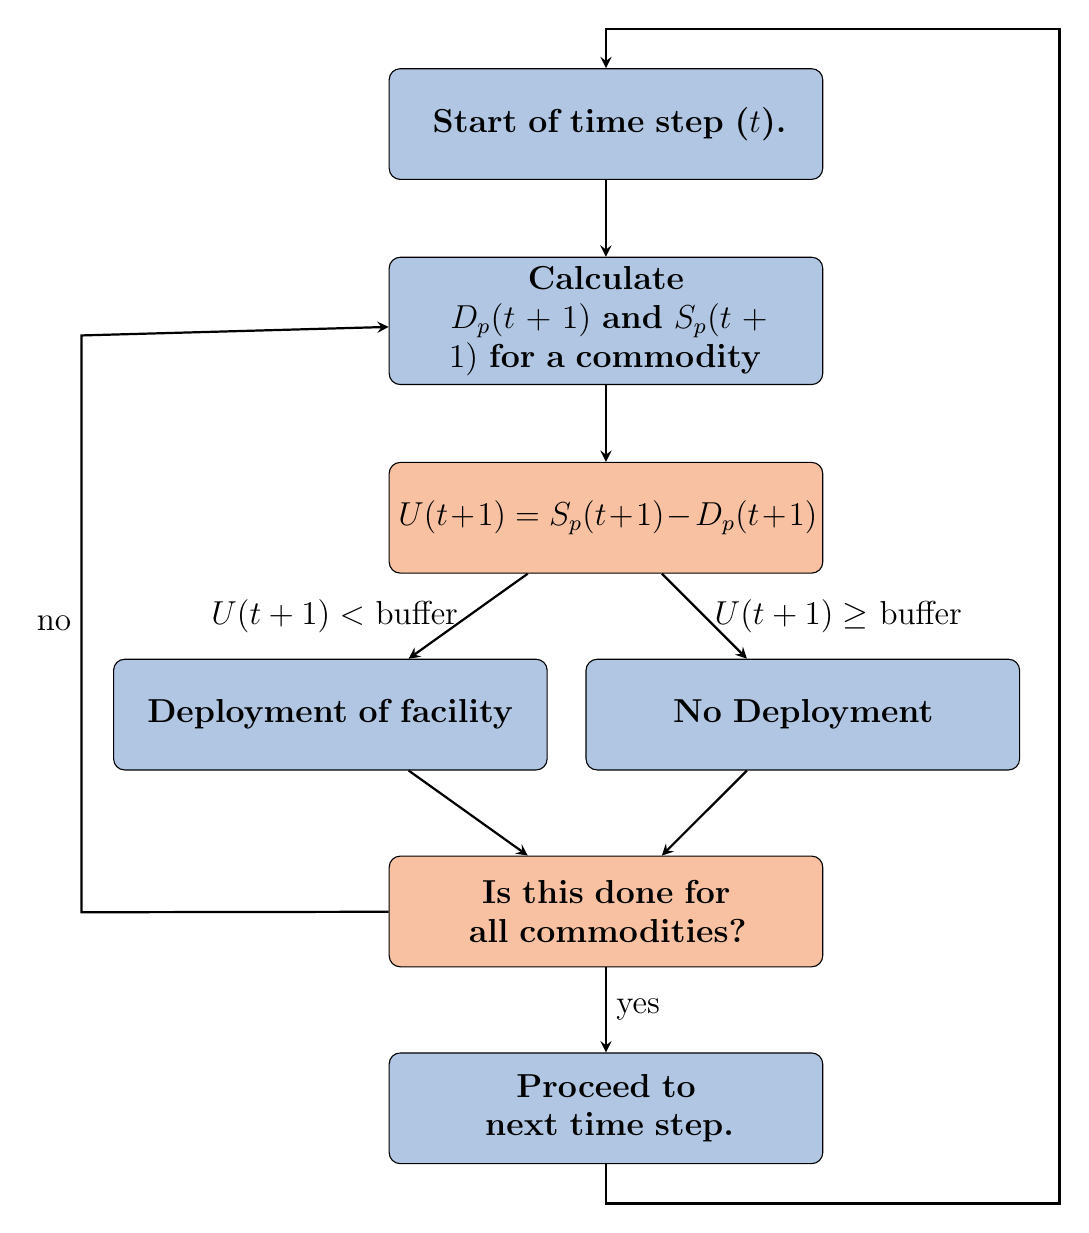
\begin{tikzpicture}[node distance=2.5cm]
    \tikzstyle{every node}=[font=\large]
	\node (Start) [bblock] {\textbf{Start of time step ($t$).}};
	\node (Predict) [bblock, below of=Start] {\textbf{Calculate \\ $D_p(t+1)$ and $S_p(t+1)$ for a commodity}};
	\node (IsThere) [oblock, below of=Predict]{\textbf{$U(t+1) = S_p(t+1)-D_p(t+1)$}};
	\node (Deploy) [bblock, below of=IsThere, xshift = -3.5cm]{\textbf{Deployment of facility}};
    \node (NoDeploy) [bblock, right of=Deploy, xshift = 3.5cm]{\textbf{No Deployment} };
    \node (All) [oblock, below of=Deploy, xshift = 3.5cm] {\textbf{Is this done for all commodities?}};
    \node (End) [bblock, below of=All] {\textbf{Proceed to next time step.}};
	
	\draw [arrow] (Start) -- (Predict); 
	\draw [arrow] (Predict) -- (IsThere);
    \draw [arrow] (IsThere) -- node[anchor=east] {$U(t+1) <$ buffer} (Deploy);
    \draw [arrow] (IsThere) -- node[anchor=west] {$U(t+1) \geq$ buffer} (NoDeploy);
    \draw [arrow] (Deploy) -- (All);
    \draw [arrow] (NoDeploy) -- (All);
    \draw [arrow] (All) -- node[anchor=west] {yes} (End);
    \draw [arrow] (All) -- ([shift={(-3.9cm,0.7cm)}]All.south west)-- node[anchor=east] {no} ([shift={(-3.9cm,-1cm)}]Predict.north west)--(Predict);
    \draw [arrow] (End) |-([shift={(3cm,-0.5cm)}]End.south east)-- ([shift={(3cm,0.5cm)}]Start.north east)-|(Start);
    \end{tikzpicture}
    \label{fig:flow}
    \caption{\Deploy logic flow at every time step in \Cyclus \cite{chee_demonstration_2019}.}
\end{figure}

\Deploy's overall objective is to ensure that there is no 
undersupply of power. 
The sub-objectives are : (1) to minimize the number of time 
steps of undersupply or under capacity of any 
commodity, (2): to minimize excessive oversupply of all commodities.
This is a reflection of reality in which it is important to 
never have an undersupply of power on the grid by ensuring power 
plants are never undersupplied of fuel, while not 
having excessive over supply resulting in a burden to store unused 
supplies. 
One of the key issues that \gls{NFCSim}s face is that despite
sufficient installed reactor capacity to meet the power 
demand, there is insufficient supply of fabricated/reprocessed 
fuel at certain time steps, resulting in idle capacity.  

\subsection{Structure}
%Description of front end and back end of fuel cycle 
%Demand Driven vs. Supply Driven 
In \deploy, two different institutions were implemented for 
front-end and back-end fuel cycle facilities: 
\texttt{DemandDrivenDeploymentInst} and 
\texttt{SupplyDriven} 
\noindent
\texttt{DeploymentInst} respectively. 
This distinction was made because front-end facilities 
are deployed to meet demand for the commodity they produce. 
Whereas, back-end facility are deployed to meet supply for the 
commodity they provide capacity for. 
For example, for front end facilities, a reactor facility 
demands fuel and \texttt{DemandDrivenDeploymentInst} 
triggers deployment of fuel fabrication facilities to create 
supply meeting demand for fuel to prevent undersupply. 
For back end facilities, the reactor generates spent fuel and 
\texttt{SupplyDrivenDeploymentInst} triggers deployment of 
waste storage facilities to create capacity meeting the supply 
of spent fuel to prevent under capacity. 

\subsection{Input Variables}
Table \ref{tab:inputs} describes the input variables that a user 
uses to customize their simulation. 
Essentially, the user must define the facilities controlled by 
\deploy, their capacities, the simulation driving commodity, 
its demand equation, deployment driving method, and which method
predicts supply and demand. 
The user also has the option to define supply/capacity buffers for 
each commodity, facility preferences, and facility constraints. 

In-depth descriptions of each input variable are found in the 
subsequent sections. 


\begin{table}[H]
	\resizebox{\textwidth}{!}{%
	\begin{tabular}{|l|l|p{7cm}|}
	\hline
											  & \textbf{Input Parameter}                                                           & \textbf{Examples}                                                                                                          \\ \hline
	\multirow{5}{*}{\textbf{Required}} & Demand driving commodity                                                           & Power, Fuel, Plutonium, etc.                                                                                                                      \\ \cline{2-3} 
											  & Demand equation                                                                    & P(t) = 10000, sin(t), 10000*t                                                                                                                 \\ \cline{2-3} 
											  & Facilities it controls                                                             & Fuel Fab, LWR reactor, SFR reactor, Waste repository, etc.                                                                                                      \\ \cline{2-3} 
											  & Capacities of the facilities                                                       & 3000 kg, 1000 MW, 50000 kg                                                                                                     \\ \cline{2-3} 
											  & Prediction algorithm                                                                  & \begin{tabular}[c]{@{}l@{}}Power: fast fourier transform\\ Fuel: moving average\\ Spent fuel: moving average\end{tabular} \\ \cline{2-3} 
											  & Deployment driven by & Installed Capacity/Supply                                                                                                                    \\ \hline
	\multirow{4}{*}{\textbf{Optional}} & Supply/Capacity Buffer type                                                                        & Absolute                                                                                                                  \\ \cline{2-3} 
											  & Supply/Capacity Buffer size                                                                        & \begin{tabular}[c]{@{}l@{}}Power: 3000 MW\\ Fuel: 0 kg \\ Spent fuel: 0 kg\end{tabular}                                   \\ \cline{2-3} 
											  & Facility preferences                                                               & \begin{tabular}[c]{@{}l@{}}LWR reactor = 100-t\\ SFR reactor = t-100 \end{tabular}          \\ \cline{2-3} 
											  & Facility constraint                                                              & SFR reactor constraint = 5000kg of Pu            \\ \hline	
			
											\end{tabular}%
	}
	\caption{\Deploy's required and optional input parameters with examples.}
	\label{tab:inputs}
	\end{table}

\subsubsection{Deployment Driving Method}
The user has the choice of deploying facilities based on difference 
between predicted demand and supply, or predicted demand and 
installed capacity. 
There are two advantages of using installed capacity over predicted 
supply. 
First, to prevent over deployment of facilities that have an
intermittent supply. 
For example, reactor facilities have a designated refueling time. 
A user might not want \deploy to deploy more reactor facilities 
to make up for the lack of power supply caused by a gap in 
supply during refueling. 
Second, to prevent infinite deployment of a facility that provides 
a commodity that is no longer available in the simulation. 
For example, in a transition scenario from \gls{LWR}s to \gls{SFR}s, 
the reprocessing plant that fabricates \gls{SFR} fuel might demand 
for Pu after the inventory accumulated by \gls{LWR}s was used up 
and there are no more \gls{LWR} facilities to generate Pu. 
This will result in \deploy deploying infinite reprocessing 
facilities to generate \gls{SFR} fuel despite the lack of Pu 
to generate the fuel. 
This can be avoided by constraining \gls{SFR} deployment until a 
sizable inventory of Pu is accumulated in the simulation. 

\subsubsection{Supply/Capacity Buffer}
In \texttt{DemandDrivenDeploymentInst}, the user has the option 
to provide a supply buffer to specific commodities so that 
\deploy will deploy facilities to meet predicted demand and the
additional buffer. 
In \texttt{SupplyDrivenDeploymentInst}, the user has the option 
to provide a capacity buffer to specific commodities so that 
\deploy will deploy facilities to meet predicted supply and the
additional buffer.
The buffer can be defined as a percentage (equation \ref{eq:perc}) 
or absolute value (equation \ref{eq:abs}). 

\begin{equation}
    \label{eq:perc}
    S_{pwb} = S_{p}*(1+d)
\end{equation}
\begin{equation}
    \label{eq:abs}
    S_{pwb} = S_{p}+a
\end{equation}
where $S_{pwb}$ is predicted supply/capacity with buffer, 
$S_p$ is the predicted supply/capacity without buffer, 
$d$ is the percentage value in decimal form, 
and $a$ is the absolute value of the buffer. 

Using a combination of this buffer capability with the 
installed capacity deployment driving method is 
effective in minimizing undersupply of a commodity without 
having excessive over supply. 
This is demonstrated in section . 

\subsection{Prediction Algorithms}
To effectively meet the objectives of \deploy, we looked to 
prediction analysis/time-forecasting techniques that are 
commonly used in other fields that use prediction analysis. 
This is a novel approach that has never been applied to 
\gls{NFCSim}s. 
\subsection{}
% Methodology: Overall objectives of d3ploy and how it works
% Structure (Demand/Supply Driven Inst)
% Input variables
% Deployment driving method (installedcap)
% Supply/Capacity Buffer 
% Prediction Methods
\FloatBarrier
\section{Results}
To demonstrate \deploy's capability to effectively conduct transition
scenario analysis and meet the objectives described in section 
\ref{sec:obj}, this section will 
(1) demonstrate \deploy's capability in simple transition scenarios, 
(2) compare the prediction methods for different transition scenarios, and
(3) demonstrate using \deploy to setup successful EG01-EG23, EG01-EG24, 
EG01-EG29, and EG01-EG30 transition scenarios. 
The input files and scripts to produce the results and plots in this
paper can be reproduced using \cite{noauthor_arfc/d3ploy:_2019}, and 
\cite{chee_arfc/transition-scenarios_2018}. 

\subsection{Demonstration of \deploy's capabilities}
\label{sec:demo}
We conducted a simple linearly increasing power demand simulation 
to demonstrate \deploy's capabilities for 
simulating transition scenarios and to inform decisions about 
input parameters when setting up larger transition scenarios 
with many facilities.
This simulation is a simple transition scenario that only includes
three facility types: \texttt{source}, \texttt{reactor}, and 
\texttt{sink}. 
The simulation initially has ten initial \texttt{reactor} facilities 
(\texttt{reactor1} to \texttt{reactor10}). 
These reactors have staggered cycle lengths and lifetimes to prevent 
simultaneous refueling and setup gradual decommissioning. 
\deploy is configured to deploy \texttt{new reactor} facilities
to meet the loss of power supply created by the decommissioning 
of the initial \texttt{reactor} facilities. 
Table \ref{tab:demonstrations} shows the \deploy input parameters 
for this simulation.  

    \begin{table}[]
        \resizebox{\textwidth}{!}{%
        \caption{\deploy's input parameters for the simple transition scenarios.}
        \label{tab:demonstrations}
        \begin{tabular}{l|l|l}
        \hline
                                  & \textbf{Input Parameters}          & \textbf{Simple Transition Scenario: Linearly Increasing Power} \\ \hline
        \multirow{5}{*}{R\textbf{equired}} & Demand driving commodity  & \multicolumn{1}{l}{Power}                            \\
                                  & Demand equation [MW]          &  $t<40 = 1000, t\geq 40 = 250t$                                                    \\
                                  & Available facilities    &  \texttt{Source}, \texttt{Reactor}, \texttt{Sink}                                                    \\
                                  & Prediction method         &  \texttt{FFT}                                                    \\
                                  & Deployment driving method & \multicolumn{1}{l}{Installed Capacity}               \\ \hline
        \multirow{2}{*}{\textbf{Optional}} & Buffer type               & \multicolumn{1}{l}{Absolute}                         \\
                                  & Buffer size               &  Power: 2000MW, Fuel: 1000kg                                                    \\ \hline
        \end{tabular}%
        }
        \end{table}

Figures \ref{fig:growingtransition-power}, \ref{fig:growingtransition-fuel}
and \ref{fig:growingtransition-spentfuel} demonstrate \deploy's capability 
to deploy reactor and supporting facilities to meet the linearly increasing
power demand and subsequently demanded secondary commodities with 
minimal undersupply.
Figure \ref{fig:growingtransition-power} demonstrates that
the main objective of \deploy was met as
there are no time steps
in which the supply of power falls under demand.
By using a combination of the \texttt{FFT} method for 
predicting demand and setting the supply buffer to 2000MW 
(the capacity of 2 reactors), the user minimizes the number of 
undersupplied time steps for every commodity.

In figure \ref{fig:growingtransition-fuel},
a source facility with a large fuel throughput is initially
deployed to meet the large initial fuel demand for the commissioning 
of ten reactors. 
By having an initial facility with a large throughput exist for the 
first few time steps, 
\deploy is prevented from deploying supporting
facilities that end up being redundant at the later times in  
the simulation.
This is a reflection of reality in which reactor manufacturers will 
accumulate an appropriate amount of fuel inventory before starting 
up reactors. 
There is one time step in which a power undersupply exists after the 
decommissioning of the large initial facility; 
this is unavoidable as the prediction methods in \deploy are 
unable to forsee this sudden drop in demand. 

\begin{figure}[]
    \centering
    \begin{subfigure}[t]{0.8\textwidth}
    \centering
        \includegraphics[width=0.9\linewidth]{figures/growingtransition-power.png} 
        \caption{The power demand is a user-defined equation and power is supplied by the reactors.
        There are no time steps with undersupply of power.}
        \label{fig:growingtransition-power}
    \end{subfigure}
    \begin{subfigure}[t]{0.6\textwidth}
        \centering
        \includegraphics[width=\linewidth]{figures/growingtransition-fuel.png} 
        \caption{Fuel is demanded by reactors and supplied by source facilities.
        There is only one time step with undersupply of fuel.}
	    \label{fig:growingtransition-fuel}
    \end{subfigure}
    \begin{subfigure}[t]{0.6\textwidth}
        \centering
        \includegraphics[width=\linewidth]{figures/growingtransition-spentfuel.png} 
        \caption{Spent Fuel is supplied by reactors and the capacity is provided by sink facilities.
        There are no time steps with under capacity of sink space.}
        \label{fig:growingtransition-spentfuel}
    \end{subfigure}
    \caption{Transition Scenario: Linearly increasing power demand.}
\end{figure}

\subsection{Comparison of Prediction Methods}

EG01-EG23, EG01-EG24, EG01-EG29, and EG01-EG30 transition scenarios
are set up in \Cyclus using \deploy. 
EG01-23 and EG01-29 transition scenario simulations have a constant 
power demand, while EG01-24 and EG01-30 have a linearly increasing
power demand. 
We identified the most effective d3ploy prediction method 
for each scenario by comparing the results of using each 
prediction method in each scenario. 
Similar to the simple transition scenario, these transition scenario 
simulations begin with an initial fleet of \glspl{LWR} 
that start progressively decommissioning at the 80-year mark, 
after which \deploy deploys \glspl{SFR} and \gls{MOX} \glspl{LWR} to meet 
the power demand. 
Figure \ref{fig:eg2329}
shows the setup of facilities and mass flows for 
EG01-23 and EG01-29 in \Cyclus. 
In EG01-23 and EG01-29, recycled plutonium from LWR spent fuel 
produces  \gls{SFR} fuel. 
EG01-24 and EG01-30 are similar to EG01-23 and EG01-29, respectively, 
with the exception that all transuranic elements are recycled.

\begin{figure}[]
	\centering
	\begin{subfigure}[t]{\textwidth}
		\centering
		\includegraphics[width=0.8\linewidth]{23flow.pdf} 
		\caption{EG01-EG23.}
		\label{fig:23flow}
	\end{subfigure}
	\vspace{1cm}
	\begin{subfigure}[t]{\textwidth}
		\centering
		\includegraphics[width=0.8\linewidth]{29flow.pdf} 
		\caption{EG01-EG29.}
		\label{fig:29flow}
	\end{subfigure}
	\hfill
	\caption{Facility and mass flow of the transition scenarios EG01-EG23 and EG01-EG29 in \Cyclus.}
	\label{fig:eg2329}
\end{figure}

In Figure \ref{fig:eg23under}, each histogram represents 
the number of time steps in each time bin with undersupply or 
under capacity for all commodities for each prediction method.  
Table \ref{tab:all-power} shows the number of time steps with power 
undersupply for constant power EG01-EG23 and EG01-29, 
linearly increasing power EG01-24 and EG01-30 transition scenarios. 
Figure \ref{fig:eg23under} demonstrates that the \texttt{POLY} method
perform the best for the EG01-23 transition scenario,
with the smallest bars on the plot, indicating that they have the 
fewest number of time steps with undersupply and under capacity
of commodities. 
We conducted a similar analysis for the constant power EG01-29 scenario,
and as seen in Table \ref{tab:all-power}, the \texttt{POLY} prediction method 
also performed best for minimizing undersupply of power.  

In Figure \ref{fig:eg24under}, each histogram represents 
the number of time steps in each time bin with undersupply or 
under capacity for all commodities for each prediction method.
Figure \ref{fig:eg24under} demonstrates that the \texttt{FFT} method 
performs the best at minimizing the undersupply of all commodities.
We conducted a similar analysis for the constant power EG01-30 scenario, and 
as seen in Table \ref{tab:all-power}, the \texttt{FFT} prediction method also performed 
best for minimizing undersupply of power. 

\begin{figure}[]
	\centering
	\includegraphics[width=1.2\linewidth]{eg01-23-histogram.png} 
	\caption{
	EG01-23 transition scenario with constant power demand. 
	Each subplot shows the total number of time steps in which there exists 
	undersupply and under capacity of commodities for each prediction method. 
	The different colors represent different commodities, and each time bin 
	refers to a specific time periods in the simulation.
	The \texttt{POLY} method performs the best, with the least number of 
	time steps with undersupply and under capacity.}
	\label{fig:eg23under}
\end{figure}

\begin{figure}[]
	\centering
	\includegraphics[width=1.2\linewidth]{eg01-24-histogram.png} 
	\caption{
	EG01-24 transition scenario with linearly increasing power demand. 
	Each subplot shows the total number of time steps in which there exists 
	undersupply and under capacity of commodities for each prediction method. 
	The different colors represent different commodities, and each time bin 
	refers to a specific time periods in the simulation.
	The \texttt{FFT} method performs the best, with the least number of 
	time steps with undersupply and under capacity.}
	\label{fig:eg24under}
\end{figure}

\begin{table}[]
	\centering
		\caption{Undersupply and oversupply of power for EG01-EG23,24,29,30 
		transition scenarios for varying prediction methods.}
		\label{tab:all-power}
		\footnotesize
        \begin{tabularx}{\textwidth}{l|RRRR}
		\hline
		& \multicolumn{3}{|c}{\textbf{Power Undersupplied Time Steps}} \\ \hline
		\textbf{Algorithm} & \textbf{EG01-EG23}  & 
		\textbf{EG01-EG24}   & \textbf{EG01-EG29} & 
		\textbf{EG01-EG30} \\ \hline
		\texttt{MA}     		    & 26 	& 36  &  15  & 24 \\ 
		\texttt{ARMA}     	    & 26 	& 36  &  15  & 24\\ 
		\texttt{ARCH}     	    &  26 	& 36  &  15  & 21\\ 
		\texttt{POLY}      		&  6 	& 65  &  4 &  9\\ 
		\texttt{EXP-SMOOTHING} 	& 27 	& 37  & 16 & 25\\ 
		\texttt{HOLT-WINTERS}  	& 27 	& 37  & 16 & 25\\ 
		\texttt{FFT}       		& 8 	& 20  & 5 & 9\\ 
		\texttt{SW-SEASONAL}    & 36 	& 107 & 14 & 51\\ \hline
	\end{tabularx}
\end{table}

From Figures \ref{fig:eg23under}, \ref{fig:eg24under}, and Table 
\ref{tab:all-power}, we can see that the \texttt{POLY} method 
performs best for constant power transition scenarios, 
and the \texttt{FFT} method performs best for linearly increasing 
power transition scenarios. 
Undersupply and under-capacity of commodities occur during two main time periods: 
initial demand for the commodity and during the transition period.
To further \deploy's primary objective of minimizing the power undersupply, 
sensitivity analysis of the power supply buffer is conducted 
with the best-performing prediction method for each transition scenario.  

\subsection{Sensitivity Analysis}
We conducted a sensitivity analysis of the power buffer size for the
EG01-EG23, EG01-24, EG01-29, and EG01-30 transition scenarios. 
Varying the power buffer size does not impact the number of 
undersupply time steps for the EG01-EG23 and EG01-EG29 constant 
power demand transition scenarios with the \texttt{POLY} prediction method.
In Table \ref{tab:all-power}, there are 6 and 4 time steps
in which there is power undersupply for the EG01-EG23 and EG01-29 
transition scenarios, respectively. 
As seen in figure \ref{fig:eg23under}, these undersupply time 
steps occur at the beginning of the simulation and for one 
time step when the transition begins. 
We expected this since without time-series data 
at the beginning of the simulation, \deploy takes a few 
time steps to collect time-series data about power demand 
to predict and start deploying reactor and supporting 
fuel cycle facilities. 
When the transition begins, power is undersupplied for one 
time step, following this, \deploy accounts for the 
undersupply by deploying facilities to meet power demand.
Therefore, we minimized the power undersupply for constant 
power EG01-EG23 and EG01-EG29 transition scenarios with 
a 0MW power supply buffer. 

We varied the power buffer size for the EG01-24 and EG01-30 
linearly increasing power demand transition scenarios. 
Figures \ref{fig:eg24-bufplot}, \ref{fig:eg30-bufplot}, 
and Table \ref{tab:buff_size} 
show that increasing the buffer size decreases the number of 
power undersupply time steps. 
For EG01-24, the cumulative undersupply plateaus at 6000MW, 
and for EG01-30, the cumulative undersupply is smallest 
for a buffer size of 8000MW.
These undersupply time 
steps occur at the beginning of the simulation and for one 
time step when the transition begins. 
We expected this since without time-series data 
at the beginning of the simulation, \deploy takes a few 
time steps to collect time-series data about power demand 
to predict and start deploying reactor and supporting 
fuel cycle facilities. 
Therefore, a buffer of 6000MW and 8000MW minimizes 
the power undersupply for EG01-EG24 and EG01-EG30, respectively.

\begin{figure}[]
	\centering
	\begin{subfigure}[t]{\textwidth}
		\centering
		\includegraphics[width=\linewidth]{24-sens-buffer.png} 
		\caption{EG01-24: Power buffer size vs. cumulative undersupply}
		\label{fig:eg24-bufplot}
	\end{subfigure}
	\begin{subfigure}[t]{\textwidth}
		\centering
		\includegraphics[width=\linewidth]{30-sens-buffer.png} 
		\caption{EG01-30: Power buffer size vs. cumulative undersupply}
		\label{fig:eg30-bufplot}
	\end{subfigure}
	\hfill
	\caption{The effect of sensitivity analysis of power buffer size on cumulative 
	undersupply of power for EG01-EG24 and EG01-EG30 transition scenarios 
	with linearly increasing power demand using the \texttt{FFT} prediction method.}
	\label{fig:sabuffer}
\end{figure}

\begin{table}[]
	\centering
	\caption{The effect of sensitivity analysis of power buffer size on cumulative 
	undersupply of power for EG01-EG24 and EG01-EG30 transition scenarios with linearly 
	increasing power demand using the \texttt{FFT} prediction method.}
	\label{tab:buff_size}
	\footnotesize
		\begin{tabular}{r|lrr}
                \hline
        \textbf{Buffer [MW]}     & \textbf{Undersupply}             & \textbf{EG01-24}   & \textbf{EG01-30} \\
		\hline
		\textbf{0}             & Time steps $[\#]$ & 20 & 9\\  
                      & Energy $[GW\cdot mo]$    & 315791 & 152517 \\ \hline
		\textbf{2000}          & Undersupplied $[\#]$ & 9 & 6 \\  
        	      & Energy $[GW\cdot mo]$    & 306520 & 147166 \\ \hline
        \textbf{4000}          & Time steps $[\#]$ & 8 & 6 \\  
				  & Energy $[GW\cdot mo]$    & 303438 & 143166 \\ \hline
		\textbf{6000}          & Time steps $[\#]$ & 7 & 5 \\  
		& Cumulative $[GW]$    & 303438 & 139083 \\ \hline
        \textbf{8000}          & Time steps $[\#]$ & 7 & 5  \\  
	              & Energy $[GW\cdot mo]$    & 303438 & 135083 \\ \hline
	\end{tabular}
\end{table}

\subsection{Best Performance Models}
Table \ref{tab:bestinputs} shows the \deploy input parameters for
EG01-EG23, EG01-EG24, EG01-EG29, and EG01-EG30 transition scenarios
that minimize the undersupply of power and 
undersupply and under-capacity of the other commodities
in the simulation. 
The need for commodity supply buffers is a reflection of reality
in which a supply buffer is usually maintained to ensure 
continuity in the event of an unexpected failure in the supply chain.

Figures \ref{fig:23stack} and \ref{fig:30stack} show
time-dependent deployment of reactor and supporting facilities for 
the EG01-23 constant power demand and EG01-30 linearly increasing power demand 
transition scenarios, respectively. 
\deploy automatically deploys reactor and supporting facilities 
to set up a supply chain to meet power demand
during a transition from \glspl{LWR} to \glspl{SFR} for EG01-23, 
and from \glspl{LWR} to \gls{MOX} \glspl{LWR} and \glspl{SFR} for 
EG01-30. 
EG01-24 and EG01-29 facility deployment plots are similar to 
EG01-23 and EG01-30, respectively, therefore they are not shown. 

\begin{table}[]
	\centering
	\begin{tabular}{r|cccc}
	\hline
	\multicolumn{1}{c|}{\multirow{2}{*}{\textbf{Input Parameter}}} & \multicolumn{4}{c}{\textbf{Simulation Description}}                                                                                                                                                                                                                                                       \\ \cline{2-5}
	\multicolumn{1}{c|}{}                                          & \multicolumn{1}{l}{\textbf{EG01-23}}                                                                 & \textbf{EG01-24}                  & \textbf{EG01-29}                 &\textbf{EG01-30}                                                  \\ \hline
	\textbf{Demand Driving}                                      & Power & Power & Power & Power                                                                                                                                                                                                                                                                                \\ 
	\textbf{Commodity} \\ \hline  
	\textbf{Demand}                                               & 60000                                                                                & 60000 & 60000                     &  60000                                        \\ 
	\textbf{Equation [MW]} & &$+250t/12$& &$+250t/12$ \\ \hline 
	\textbf{Prediction}                                             & \texttt{POLY}       & \texttt{FFT}             & \texttt{POLY}         &  \texttt{FFT}    \\ 
	\textbf{Method} \\ \hline 
	\textbf{Deployment}   & Installed & Installed  & Installed   & Installed    \\                                                                                                                                                                                 
	\textbf{Driving Method} & Capacity & Capacity  & Capacity   & Capacity \\ \hline 
	\textbf{Fleet Share} &  MOX: 85\% &  MOX: 85\% &  MOX: 85\% &  MOX :85\%     \\
	\textbf{Percentage} &SFR: 15\%&SFR: 15\%&SFR: 15\%&SFR: 15\%\\ \hline
	\textbf{Buffer type}                                                    & \multicolumn{4}{c}{Absolute}                                                                                                                                                                                                                                                               \\ \hline
	\textbf{Power Buffer}                                                  & 0 & 6000 & 0 & 8000 \\ 
	\textbf{Size [MW]} \\ \hline \end{tabular}
	\caption{\deploy's input parameters for EG01-EG23, EG01-EG24, EG01-EG29, and 
	EG01-EG30 transition scenarios
	that minimizes undersupply of power and minimizes 
	the undersupply and under-capacity of the other facilities. }
	\label{tab:bestinputs}
	\end{table}

\begin{figure}[]
	\centering
	\begin{subfigure}[t]{1.2\textwidth}
		\centering
		\includegraphics[width=\linewidth]{eg23-stack_reactor.png} 
		\caption{EG01-23: Reactor Deployment}
		\label{fig:23reactor}
	\end{subfigure}
	\vspace{1cm}
	\begin{subfigure}[t]{1.2\textwidth}
		\centering
		\includegraphics[width=\linewidth]{eg23-stack_support.png} 
		\caption{EG01-23: Supporting Facility Deployment}
		\label{fig:23support}
	\end{subfigure}
	\hfill
	\caption{Time dependent deployment of reactor and supporting facilities in 
	the EG01-23 constant power demand transition scenario. 
	\deploy automatically deploys reactor and supporting facilities 
	to setup a supply chain to meet constant power demand of $60000$ MW
	during a transition from \glspl{LWR} to \glspl{SFR}. }
	\label{fig:23stack}
\end{figure}

\begin{figure}[]
	\centering
	\begin{subfigure}[t]{1.2\textwidth}
		\centering
		\includegraphics[width=\linewidth]{eg30-stack_reactor.png} 
		\caption{EG01-30: Reactor Deployment}
		\label{fig:30reactor}
	\end{subfigure}
	\vspace{1cm}
	\begin{subfigure}[t]{1.2\textwidth}
		\centering
		\includegraphics[width=\linewidth]{eg30-stack_support.png} 
		\caption{EG01-30: Supporting Facility Deployment}
		\label{fig:30support}
	\end{subfigure}
	\hfill
	\caption{Time dependent deployment of reactor and supporting facilities in 
	the EG01-30 linearly increasing power demand transition scenario. 
	\deploy automatically deploys reactor and supporting facilities 
	to setup a supply chain to meet linearly increasing power demand of $60000 + 250t/12$ MW
	during a transition from \glspl{LWR} to MOX LWRs and \glspl{SFR}. }
	\label{fig:30stack}
\end{figure}

\begin{table}[]
	\centering
        \caption{Undersupply/capacity of key commodities for the best performing EG01-EG23,24,29,30 transition scenarios.}
		\label{tab:all-power}
		\footnotesize
        \begin{tabular}{lcccc}
		\hline
		& \multicolumn{3}{c}{\textbf{No. of Time Steps with Undersupply}} \\ \hline
		\textbf{Transition Scenario} & EG01-EG23 & 
		EG01-EG24 & EG01-EG29 & EG01-EG30 \\ \hline 
		\textbf{Commodities} \\ 
		Natural Uranium		    & 2 	& 3  &  1  & 1 \\ 
		\gls{LWR} Fuel     	    & 4 	& 6  &  1  & 2\\ 
		\gls{SFR} Fuel     	    &  0 	& 0  &  2  & 2\\ 
		\gls{MOX} \gls{LWR} Fuel &-&-&2&2 \\
		Power      				&  6 	& 7  &  4 &  5\\ 
		\gls{LWR} Spent Fuel	& 1 	& 1  & 1 & 1\\ 
		\gls{SFR} Spent Fuel     	    &  1 	& 1  &  1  & 1\\ 
		\gls{MOX} \gls{LWR} Spent Fuel &-&-&1&1 \\ \hline 
	\end{tabular}
\end{table}

% demonstration of d3ploy's capabilities (basic transition cases) 
% comparison of prediction methods
% - Tables: table 10 from report + more buffer size steps, 
% - Example model   
\FloatBarrier
\section{Conclusion}
The present nuclear fuel cycle in the United States is a once-through 
fuel cycle of LWRs with no used fuel reprocessing. 
This nuclear fuel cycle faces cost, safety, proliferation, and spent 
nuclear fuel challenges that hinder large-scale nuclear power deployment. 
The U.S Department of Energy identified future 
nuclear fuel cycles, involving continuous recycling of co-extracted U/Pu or 
U/TRU in fast and thermal spectrum reactors, that may overcome these challenges.
These transition scenarios have been modeled previously in the following 
nuclear fuel cycle simulators \cite{feng_standardized_2016,bae_standardized_2019}: 
ORION, DYMOND, VISION, MARKAL, and \Cyclus. 
However, for many nuclear fuel cycle simulators, the user is required to 
define a deployment scheme for all supporting facilities to avoid any 
supply chain gaps or resulting idle reactor capacity. 
Manually determining a deployment scheme for a once-through 
fuel cycle is straightforward; however, for complex fuel cycle 
scenarios, it is not. 
In this paper, we introduce the capability, \deploy, in \Cyclus 
that automatically deploys 
fuel cycle facilities to meet user-defined power demand.     
In this paper, we demonstrate that with careful selection of 
\deploy parameters, we can 
completely automate the setup of constant and 
linearly increasing power demand transition scenarios
for EG01-23, EG01-24, EG01-29, and EG01-30 with minimal 
power undersupply. 
Using \deploy to set up transition scenarios 
saves the user simulation set-up time, making it more efficient 
than the previous efforts that
required a user to manually calculate and use trial and error 
to set up the deployment scheme for the supporting fuel cycle 
facilities. 
Transition scenario simulations set up manually are sensitive 
to changes in the input parameters resulting in an 
arduous setup process since a slight change in one 
input parameter would result in the need to recalculate 
the deployment scheme to ensure no undersupply 
of power.   
Therefore, by automating this process, when the user varies input parameters 
in the simulation, \deploy automatically adjusts the
deployment scheme to meet the new constraints. 
\FloatBarrier
\section{Future Work}
We simulate transition scenarios to predict the future; 
however, when implemented in the real world, the transition 
scenario tends to deviate from the optimal scenario.
Therefore, nuclear fuel cycle simulators must be used to conduct
sensitivity analysis studies to understand the subtleties of 
a transition scenario better to reliably inform policy decisions.
Previously it was difficult to conduct sensitivity analysis with \Cyclus 
as users have to manually calculate the deployment scheme for a 
single change in an input parameter. 
By using the \deploy capability,
sensitivity analysis studies are more efficiently 
conducted as facility deployment in transition scenarios 
are automatically set up. 
\deploy will also be open-source and available for the forseeable future on github 
\cite{chee_arfc/d3ploy:_2019}, to be used with \Cyclus for conducting any 
transition scenario analysis. 
The transition scenario simulations in this work assume recipe reactors, 
however, in reality, complexity introduced by the reprocessing plants causes 
each reactor to have dynamic incoming and outgoing material compositions. 
Therefore, the static recipe method assumption is a poor approximation 
\cite{bae_neural_2019,peterson-droogh_value_2018}. 
In future transition scenario work with \deploy, a \Cyclus 
reactor archetype that uses dynamic fuel compositions could be used. 

\FloatBarrier
\section{Acknowledgments}
\gls{DOE} Office of Nuclear Energy funds this research through 
the  Nuclear Energy University Program (Project 16-10512, DE-NE0008567) 
`Demand-Driven Cycamore Archetypes'. The authors want to thank 
members of the \gls{ARFC} group at the University of Illinois at 
Urbana-Champaign. 
Special thanks to Kip Kleimenhagen and Matthew Kozak 
for their excellent proofreading help. 
We also thank our colleagues from the \Cyclus community
for collaborative \Cyclus development.

The authors contributed to this work as described below. 
Gwendolyn J. Chee conceived and designed the simulations, wrote the paper, 
prepared figures and/or tables, performed the computation work, contributed to
and validated the software product, and reviewed drafts of the paper. 
Roberto E. Fairhurst Agosta performed the computation work and contributed to
the software product. 
Jin Whan Bae conceived and designed the simulations and contributed to and validated
the software product. 
Robert R. Flanagan conceived and designed the simulations and contributed to 
the software product. 
Anthony M. Scopatz conceived and designed the simulations and acquired funding 
support for the project. 
Kathryn D. Huff directed and supervised the work, acquired funding 
support for the project, conceived and designed the simulations, contributed to 
the software product, and reviewed drafts of the paper.
\FloatBarrier

%\nocite{robertson_conceptual_1971} % placeholder until citations appear
\bibliography{2019-ddca}

%%% Random thoughts 
% deploy vs Deploy?

\end{document}
